\documentclass[final]{beamer}
\setbeamertemplate{navigation symbols}{}
\usepackage[size=a0,scale=1.55]{beamerposter}
\usetheme{Berlin}

\usepackage{graphicx} 

\usepackage{pgfplotstable} 
\usepackage{pgfplots}
\pgfplotsset{compat=1.17}

\usepackage{caption}

\usepackage[utf8]{inputenc}
\usepackage[T1]{fontenc}
\usepackage[scale=0.8]{newpxtext} 

\usepackage{tikz}
\usetikzlibrary{shapes, arrows.meta, positioning}

\title{Statistics: Unlocking the Power of Data}
\author{Group 9}
\institute{Target audiences: A-Level students}
\date{\today}

\begin{document}

\begin{frame}[t]{}

	\vspace{-0.6cm}

	\begin{columns}[t]
		
		% Column 1
		\begin{column}{.3\textwidth}

			\begin{block}{What is Statistics?}

				Statistics is the science of learning from data. It enables us to understand patterns and make decisions based on data analysis.

				\vspace{1cm}

				For example, by examining the variability in A-Level mathematics results between summer 2020 and summer 2021, we can gain insights into how the pandemic might have affected student performance and assessment methods. This understanding can then inform educational strategies and policies.

				\vspace{1cm}

				\begin{figure}
					
					\begin{tikzpicture}

						\begin{axis}[
								name=myaxis,
								ybar,
								bar width=10pt,
								width=20cm,
								height=15cm,
								xlabel={Change in centre percentage of grade A or above},
								ylabel={Number of centres},
								xlabel style={font=\footnotesize},
								ylabel style={font=\footnotesize},
								tick label style={font=\tiny},
								legend style={font=\tiny},
								xmin=-50, xmax=50,
								ymin=0, ymax=170,
								xtick={-50,-40,...,50},
								ytick={0,50,...,200},
								legend pos=north east,
								ymajorgrids=true,
								grid style=dashed,
							]

							\addplot[
								fill=purple,
								draw=black,
							] coordinates {
									(-33.75, 1)
									(-31.25, 1)
									(-28.75, 1)
									(-26.25, 3)
									(-23.75, 5)
									(-21.25, 7)
									(-18.75, 12)
									(-16.25, 14)
									(-13.75, 27)
									(-11.25, 40)
									(-8.75, 41)
									(-6.25, 56)
									(-3.75, 80)
									(-1.25, 108)
									(1.25, 114)
									(3.75, 127)
									(6.25, 111)
									(8.75, 110)
									(11.25, 79)
									(13.75, 72)
									(16.25, 48)
									(18.75, 37)
									(21.25, 23)
									(23.75, 20)
									(26.25, 12)
									(28.75, 13)
									(31.25, 3)
									(33.75, 6)
									(36.25, 3)
									(41.25, 1)
									(43.75, 2)
									(46.25, 1)
									(48.75, 1)
								};
						\end{axis}

						\footnotesize\node[align=left,anchor=west] at ([xshift=1cm]myaxis.east) {
							Number of centres = 1179\\
							Mean = 4.3\\
							Standard Deviation = 10.9
						};

					\end{tikzpicture}

					\caption{Variability in A-Level mathematics results – summer 2020 vs. summer 2021.}
					\caption*{\textit{\centering\scriptsize Data source: UK Government's Department for Education}}

				\end{figure}

				\vspace{0.5cm}
				
			\end{block}

			\vspace{0.5cm}

			\begin{block}{Engaging Advanced Concepts}

				\vspace{2cm}

				\begin{minipage}{0.3\textwidth}
					\centering
					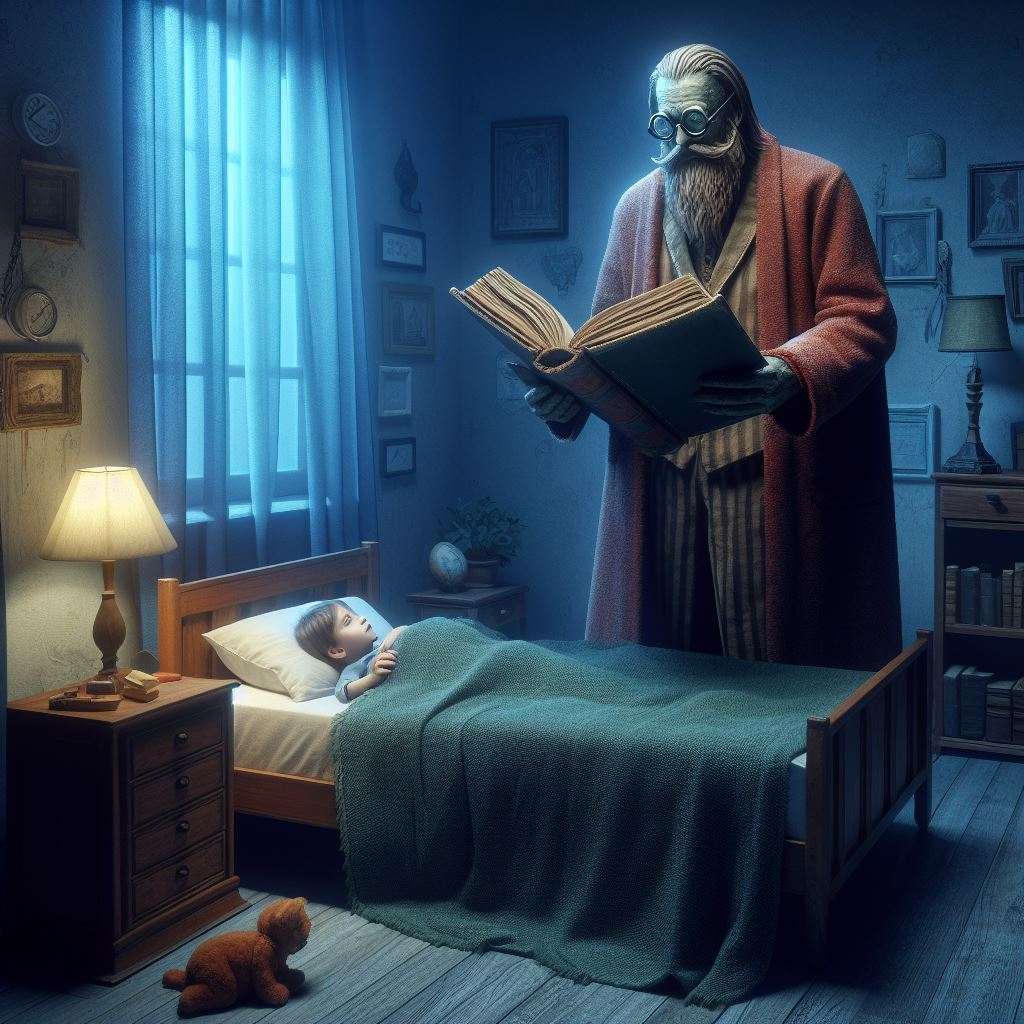
\includegraphics[width=\linewidth]{./images/1-2-1-StoryTelling.jpeg}
				\end{minipage}
				\hfill
				\begin{minipage}{0.68\textwidth}
					\textbf{Descriptive Statistics \& Inferential Statistics:} Think of statistics as storytelling. Descriptive statistics outline the story - the heroes and their journey. Inferential statistics predict the next twist, based on the story so far.
				\end{minipage}

				\vspace{1cm}

				\begin{minipage}{0.3\textwidth}
					\centering
					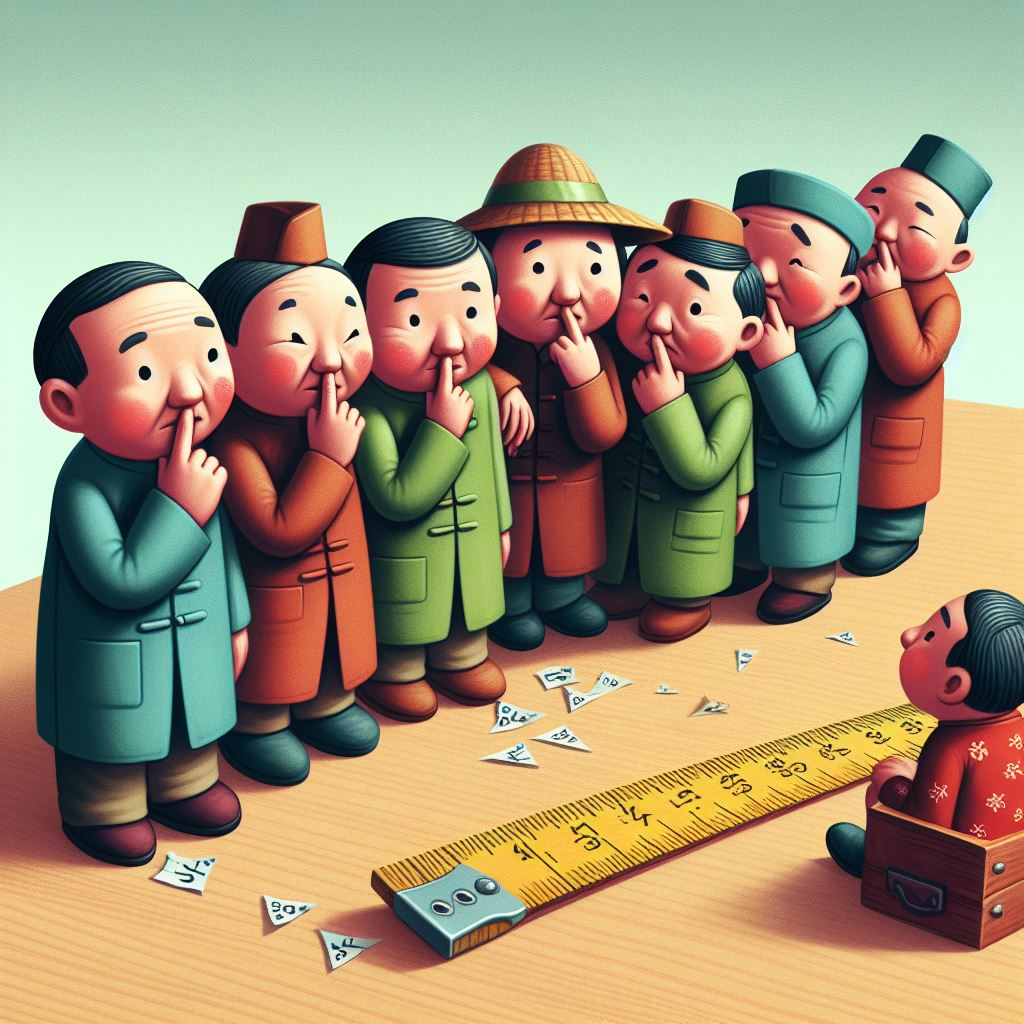
\includegraphics[width=\linewidth]{./images/1-2-2-WhisperGame.jpeg} 
				\end{minipage}
				\hfill
				\begin{minipage}{0.68\textwidth}
					\textbf{Error Propagation:} Like a game of telephone, small errors in measurements can grow when combined. Understanding this helps us make decisions with the most accurate information.
				\end{minipage}

				\vspace{1cm}

				\begin{minipage}{0.3\textwidth}
					\centering
					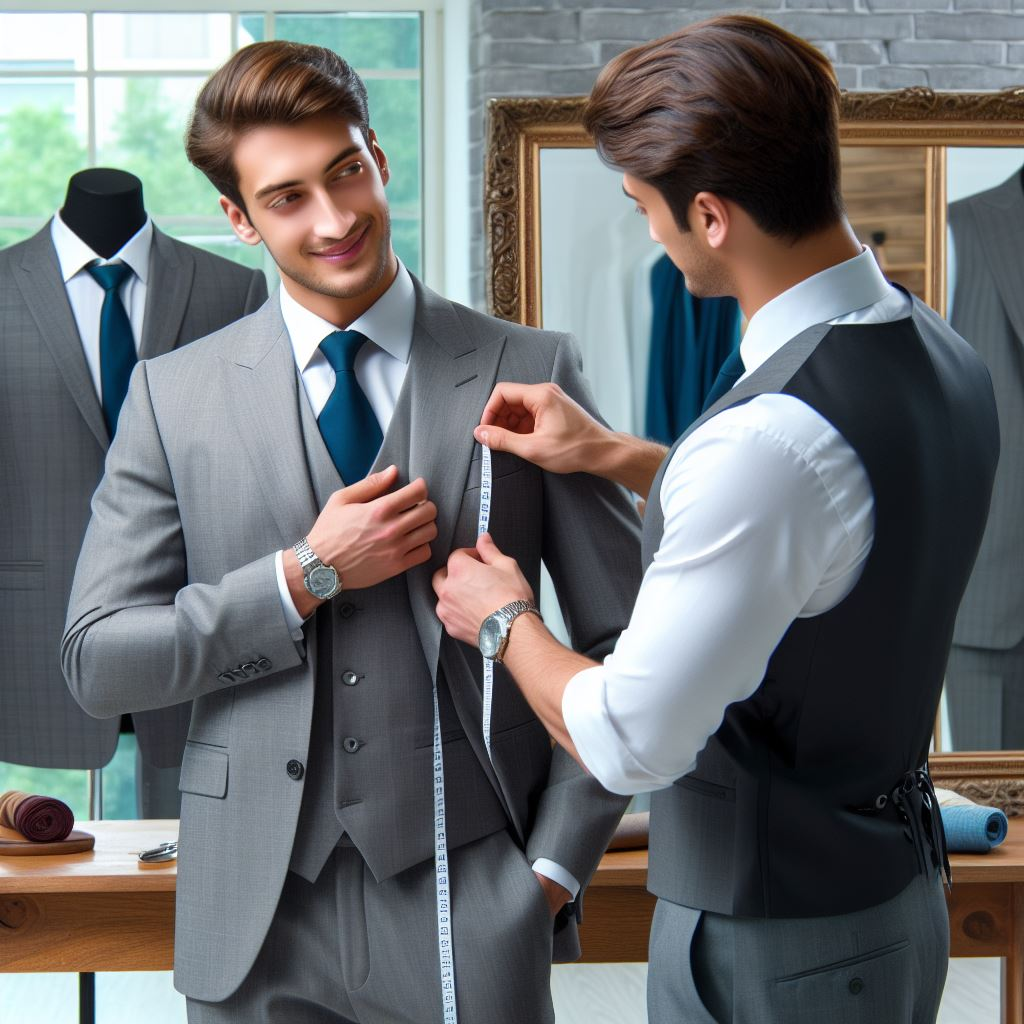
\includegraphics[width=\linewidth]{./images/1-2-3-TailorSuit.jpeg}
				\end{minipage}
				\hfill
				\begin{minipage}{0.68\textwidth}
					\textbf{Model Fitting and Confidence:} Like tailoring a suit, we adjust our models to fit our data. Confidence tells us how sure we can be about our predictions.
				\end{minipage}

				\vspace{1.75cm}

			\end{block}

		\end{column}

		% Column 2 - centre - title block
		\begin{column}{.33\textwidth}

			\vspace{-0.6cm}

			\begin{block}{}
				\centering
				\Large \textbf{\inserttitle}\\

				\vspace{1cm}

				\normalsize \insertauthor\\

				\vspace{1cm}

				\small \textit{\insertinstitute}\\

				\vspace{1cm}

			\end{block}

			\vspace{0.5cm}

			\begin{block}{The Fascinating World of Statistics: Why It Matters \& How It's Used}

				Statistics is more than just numbers and graphs. It's the backbone of decision-making in our daily lives, science, and business.

				\vspace{0.5cm}

				Here's how statistics lights up the path in various fields, making the complex simple and the uncertain clear:

				\vspace{1cm}

				\begin{minipage}{0.3\textwidth}
					\centering
					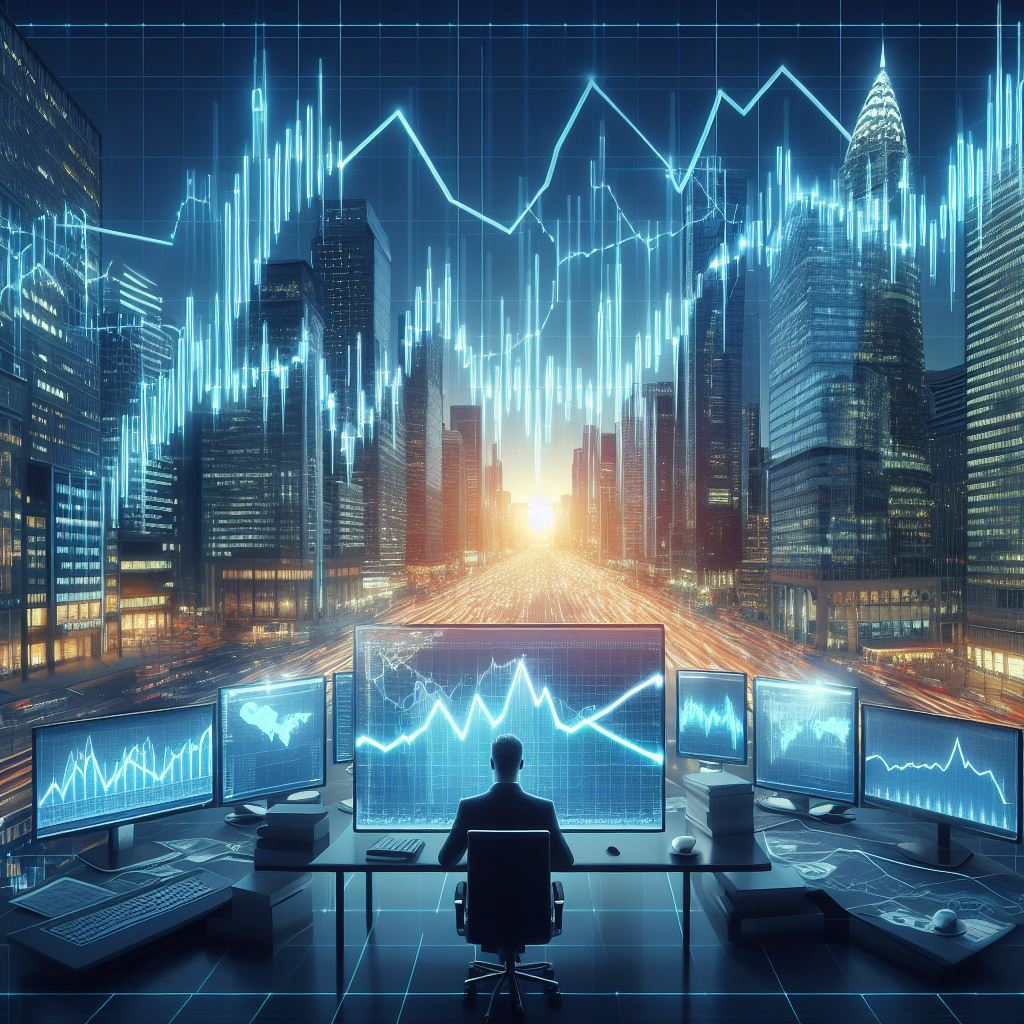
\includegraphics[width=0.88\linewidth]{./images/2-2-1-StockMarket.jpeg}
				\end{minipage}
				\hfill
				\begin{minipage}{0.68\textwidth}
					\textbf{In Economics:} Ever wondered how stock markets predict future trends? Statistics! By analyzing past data, statisticians can forecast market movements, helping investors make informed decisions.
				\end{minipage}

				\vspace{1cm}

				\begin{minipage}{0.3\textwidth}
					\centering
					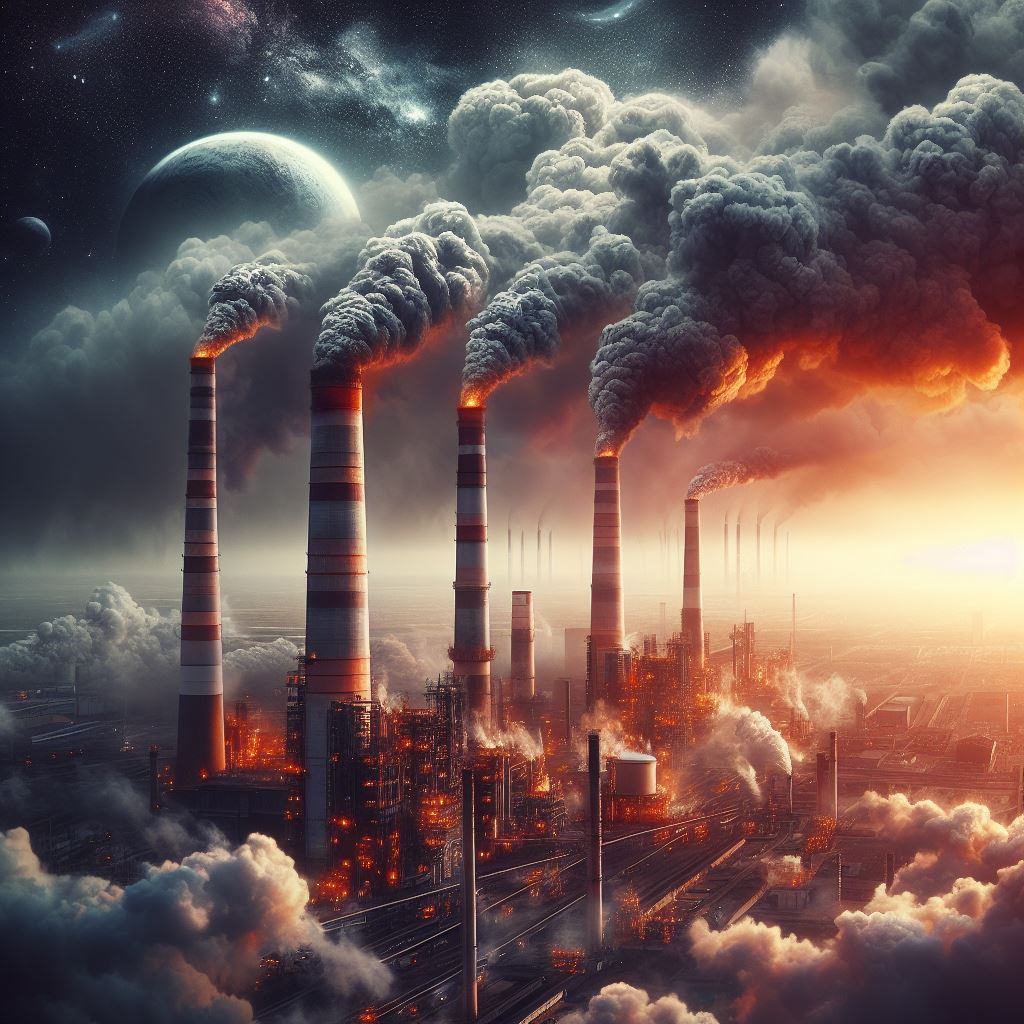
\includegraphics[width=0.88\linewidth]{./images/2-2-2-AirPollution.jpeg}
				\end{minipage}
				\hfill
				\begin{minipage}{0.68\textwidth}
					\textbf{In Environmental Science:} How do we know if the air quality is getting worse or better? Through statistics, scientists track pollution levels over time, providing us with information to protect our planet.
				\end{minipage}

				\vspace{1cm}

				\begin{minipage}{0.3\textwidth}
					\centering
					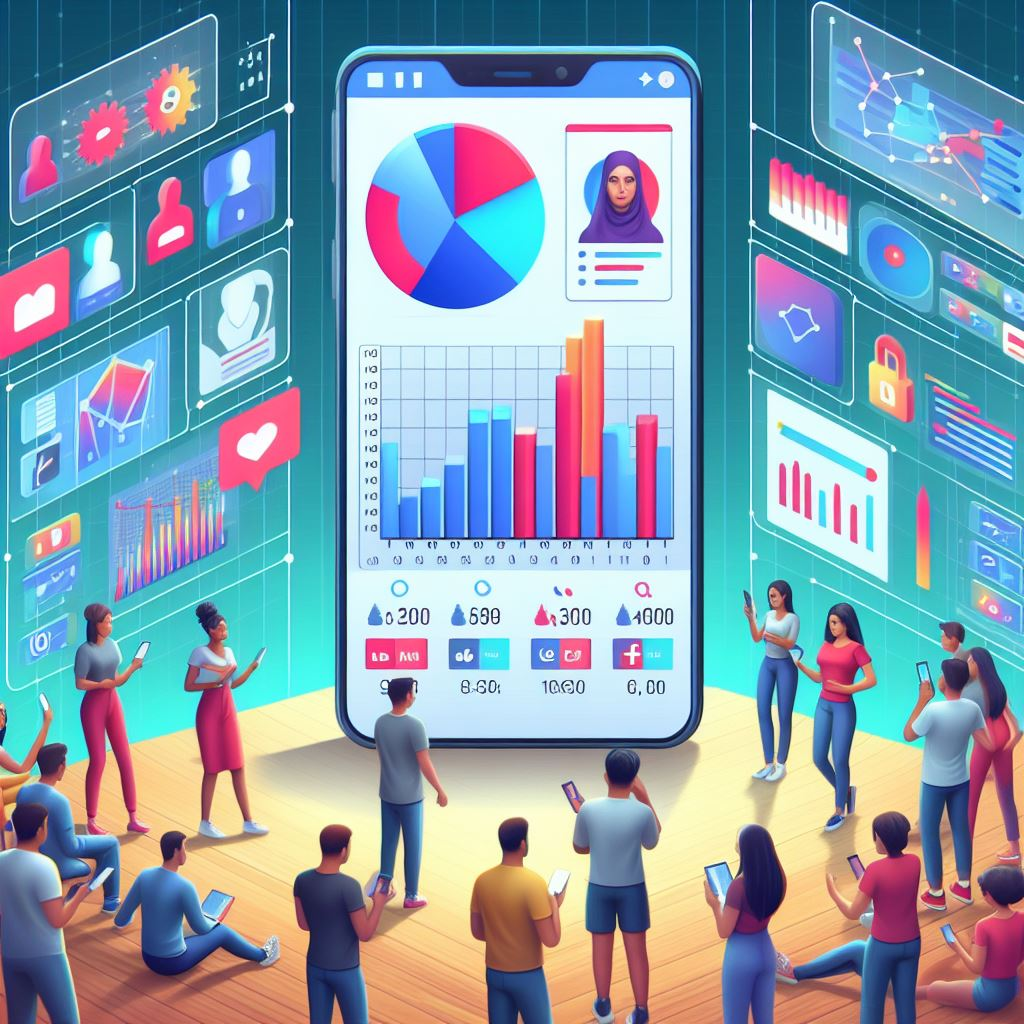
\includegraphics[width=0.88\linewidth]{./images/2-2-3-SocialMedia.jpeg}
				\end{minipage}
				\hfill
				\begin{minipage}{0.68\textwidth}
					\textbf{In Social Media Analysis:}  Ever noticed how some posts get more likes or shares than others? That's statistics at work! By analyzing data on user engagement (like clicks, shares, and time spent on posts), content creators can optimize their posts to reach a wider audience.
				\end{minipage}

				\vspace{1cm}

			\end{block}

			\vspace{0.5cm}
			
			\begin{block}{A World Without Statistics}
				
				\vspace{1cm}
				
				\begin{minipage}{0.43\textwidth}
					\centering
					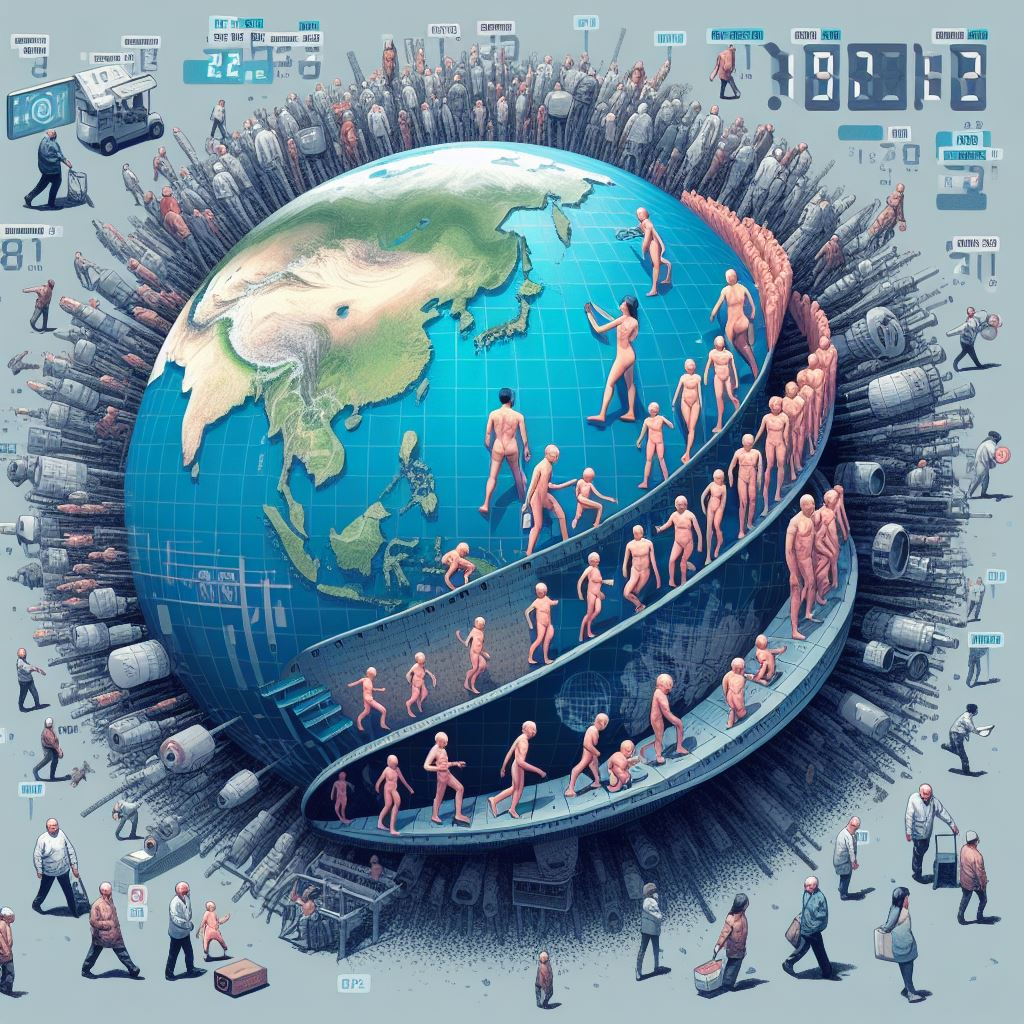
\includegraphics[width=0.7\linewidth]{./images/2-3-1-PopulationOverload.jpeg}\\
					\vspace{0.5cm}  
					\textbf{Population Overload}\\
					\small Without statistics, we can't analyze or predict population trends, risking unsustainable growth.
				\end{minipage}
				\hfill
				\begin{minipage}{0.43\textwidth}
					\centering
					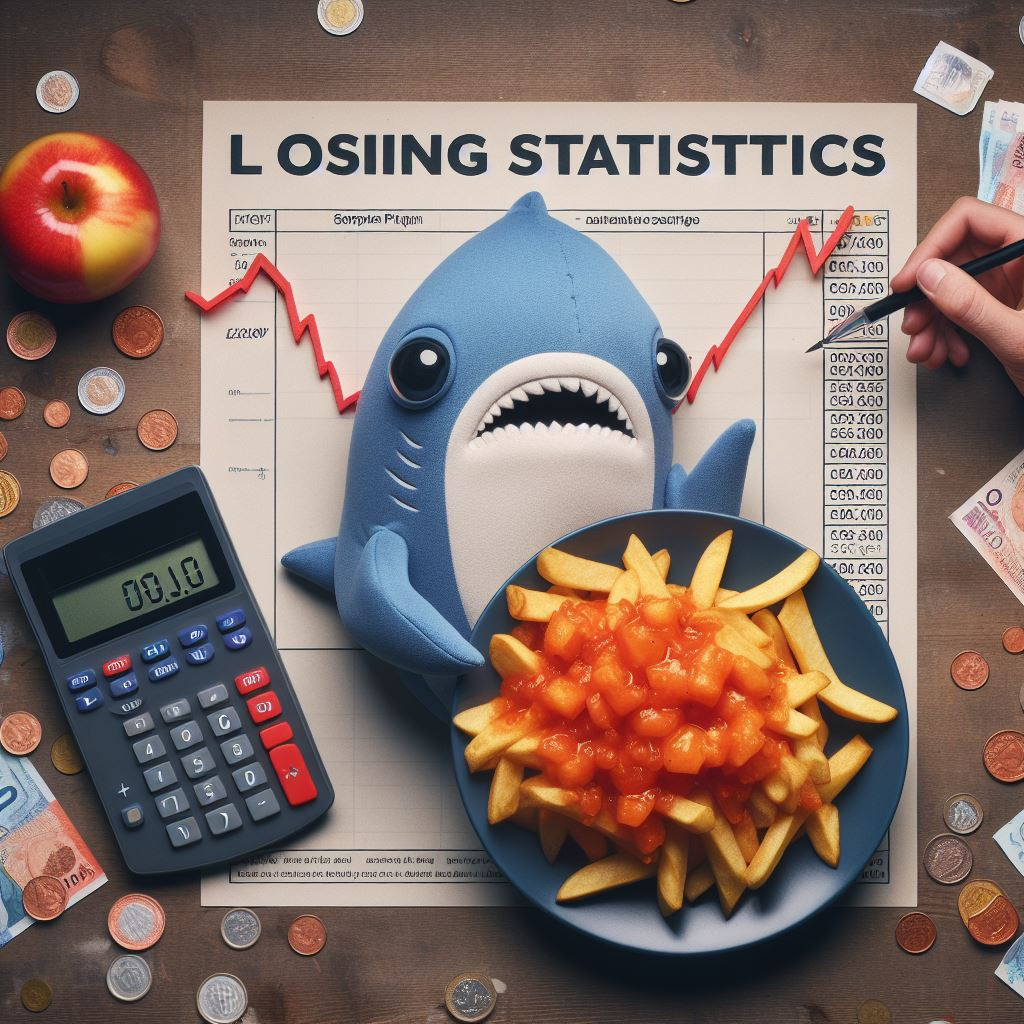
\includegraphics[width=0.7\linewidth]{./images/2-3-2-Inflation.jpeg}\\
					\vspace{0.5cm}  
					\textbf{Inflation Out of Control}\\
					\small Without statistics, controlling inflation is a guesswork. Imagine paying £1,000 for fish and chips!
				\end{minipage}

				\vspace{0.5cm}
				
			\end{block}
			
		\end{column}

		% Column 3
		\begin{column}{.3\textwidth}

			\begin{block}{Making Statistics Fun with Data Visualization}

				\vspace{0.5cm}

				Let's dive into how sports teams, like \textbf{Ross Venus}'s ice hockey team, use statistics and data visualization to scout talent and predict game outcomes. By analyzing player performance data over the season, teams can create visual representations to compare players, predict future performance, and make strategic decisions.

				\vspace{0.5cm}

				It's not just about the goals. It's about understanding the player's journey and potential through the lens of data.

				\vspace{1cm}

				\begin{figure}[htbp]
					
					\centering
					
					\begin{minipage}[t][0.4\textwidth][t]{0.3\textwidth}
						\hspace*{5mm}
						\vspace{0cm}
						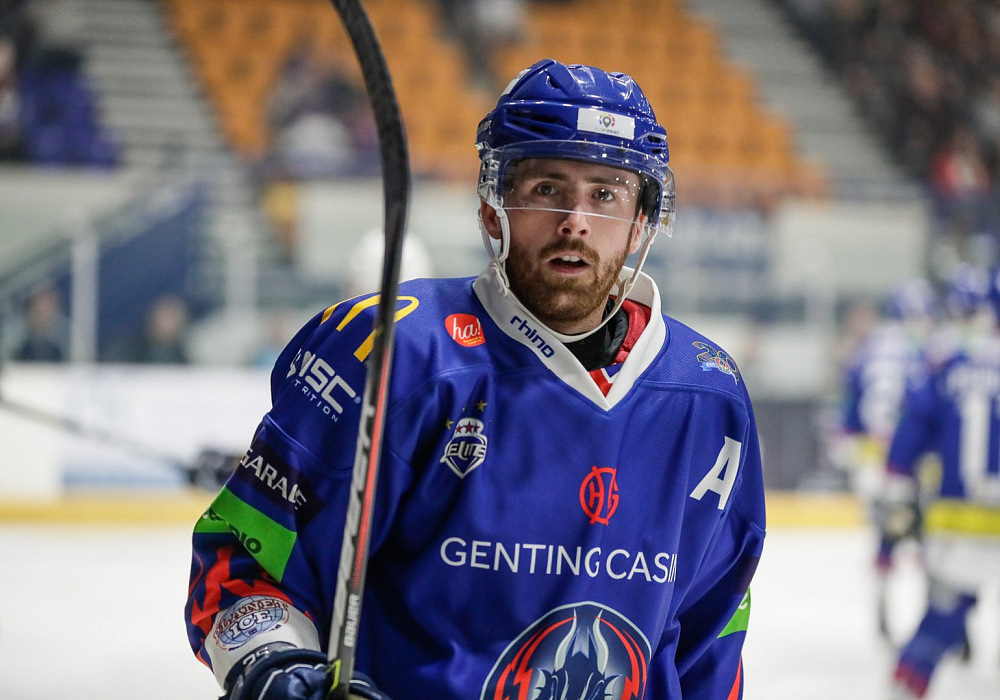
\includegraphics[width=0.9\linewidth]{./images/3-1-1-RossVenus}
						\caption{Ross Venus}
						\vspace{-0.3cm}
						\caption*{\textit{\centering\scriptsize Photo: Scott Wiggins}}
					\end{minipage}
					\hfill
					\begin{minipage}{0.65\textwidth}
						\vspace{-2cm}
						\begin{table}
							\centering
							\caption{Scoring Data for Ross Venus}
							{\footnotesize
								\begin{tabular}{|l|l|l|l|l|l|l|}
									\hline
									Season  & Team                    & League        & GP & G  & A  & TP \\ \hline
									2006-07 & Coventry Blaze U16      & England U16   & 7  & 0  & 3  & 3  \\
									2007-08 & Coventry Blaze U16      & England U16 2 & 9  & 9  & 16 & 25 \\
									2008-09 & Coventry Blaze U16      & England U16   & 14 & 14 & 16 & 30 \\
									2009-10 & Coventry Blaze U16      & England U16   & 15 & 42 & 16 & 58 \\
									2021-22 & Coventry Blaze          & EIHL          & 54 & 8  & 21 & 29 \\
									2022-23 & Coventry Blaze          & EIHL          & 53 & 9  & 23 & 32 \\
									2023-24 & Milton Keynes Lightning & NIHL          & 36 & 27 & 55 & 82 \\ \hline
								\end{tabular}
							}
						\end{table}
					\end{minipage}
					
				\end{figure}

				\vspace{-3cm}

				\begin{figure}[ht]
					
					\centering
					
					\begin{tikzpicture}
						
						\begin{axis}[
								title={},
								xlabel={Season},
								xlabel style={font=\footnotesize},
								ylabel={Scores},
								ylabel style={font=\footnotesize},
								width=30cm,
								height=11.2cm,
								symbolic x coords={2006-07,2007-08,2008-09,2009-10,2021-22,2022-23,2023-24},
								xtick=data,
								tick label style={font=\tiny},
								legend style={font=\tiny},
								legend pos=north west,
								ymajorgrids=true,
								grid style=dashed,
							]

							\addplot[mark=*,violet] coordinates {
									(2006-07,3)
									(2007-08,25)
									(2008-09,30)
									(2009-10,58)
									(2021-22,29)
									(2022-23,32)
									(2023-24,82)
								};

							\addlegendentry{Total Points}

							\addplot[mark=square*,cyan] coordinates {
									(2006-07,0)
									(2007-08,9)
									(2008-09,14)
									(2009-10,42)
									(2021-22,8)
									(2022-23,9)
									(2023-24,27)
								};

							\addlegendentry{Goals}

							\addplot[mark=triangle*,black] coordinates {
									(2006-07,3)
									(2007-08,16)
									(2008-09,16)
									(2009-10,16)
									(2021-22,21)
									(2022-23,23)
									(2023-24,55)
								};

							\addlegendentry{Assists}
						\end{axis}
						
					\end{tikzpicture}

					\caption{Scoring Trends of Ross Venus Across Different Seasons}
					\caption*{\textit{\centering\scriptsize Data source: Elite Prospects}}

				\end{figure}

				\vspace{0.5cm}

			\end{block}
			
			\vspace{0.5cm}
			
			\begin{block}{Data Visualization Journey}
				
				\vspace{2cm}
				\centering
				
				\begin{tikzpicture}
					
					\tikzstyle{icon} = [minimum width=5cm, minimum height=2cm, node distance=8cm]
					\tikzstyle{description} = [text width=13cm, align=center, node distance=1cm]
					\tikzstyle{arrow} = [thick,->,>=stealth]
					\tikzstyle{number} = [circle, fill=white, draw, font=\bfseries]
					
					\node[icon] (collecting) {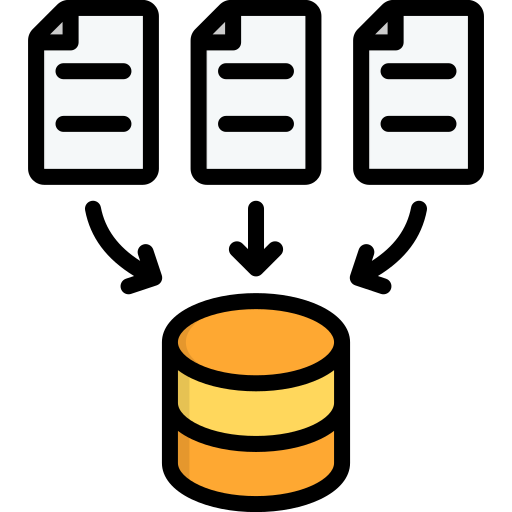
\includegraphics[width=5cm]{./images/3-2-1-DataCollect.png}};
					\node[icon, right=of collecting] (analysis) {
\includegraphics[width=5cm]{./images/3-2-2-DataAnalysis.png}};
					\node[icon, below=of collecting] (visualization) {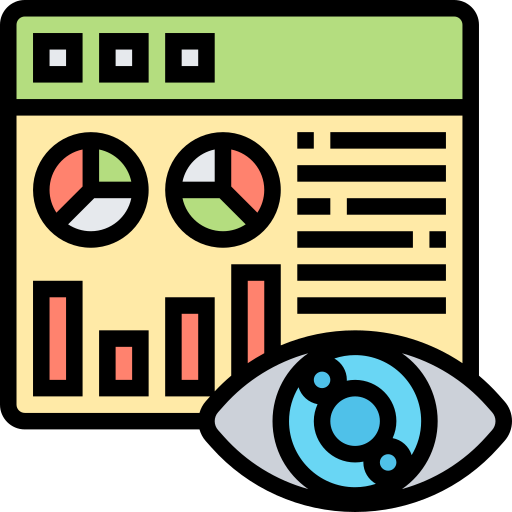
\includegraphics[width=5cm]{./images/3-2-3-DataVisualize.png}};
					\node[icon, right=of visualization] (decision) {
\includegraphics[width=5cm]{./images/3-2-4-DecisionMaking.png}};
					
					\node[description, below=of collecting] (desc1) {\textbf{Collecting Data}\\Gathering\\ performance metrics};
					\node[description, below=of analysis] (desc2) {\textbf{Analysis}\\Identifying trends and patterns};
					\node[description, below=of visualization] (desc3) {\textbf{Visualization}\\Creating visual representations};
					\node[description, below=of decision] (desc4) {\textbf{Decision Making}\\Informing\\ strategic decisions};
					
					\node[number] at ([xshift=-2cm]collecting.west) (num1) {1};
					\node[number] at ([xshift=-2cm]analysis.west) (num2) {2};
					\node[number] at ([xshift=-2cm]visualization.west) (num3) {3};
					\node[number] at ([xshift=-2cm]decision.west) (num4) {4};

				\end{tikzpicture}

				\vspace{1.8cm}
				
			\end{block}

		\end{column}
		
	\end{columns}
	
\end{frame}

\end{document}